%% LaTeX2e class for student theses
%% sections/conclusion.tex
%% 
%% Karlsruhe Institute of Technology
%% Institute for Program Structures and Data Organization
%% Chair for Software Design and Quality (SDQ)
%%
%% Dr.-Ing. Erik Burger
%% burger@kit.edu
%%
%% Version 1.1, 2014-11-21

\chapter{Verwandte Arbeiten}
\label{ch:verwandteArbeiten}

Im Folgenden wird der aktuelle Forschungsstand bzgl. Datenflussanalysen auf Architekturebene beschrieben. Dabei werden Arbeiten vorgestellt, die als Grundlage dieser Bachelorarbeit dienen, bzw. von denen sich diese Arbeit abgrenzt. 

\section{Vertraulichkeitsbegriffsbildung}
\label{sec:vertraulichkeit}
Zunächst muss ein Vertaulichkeitsbegriff gefunden werden, der sich auf Architekturebene überprüfen lässt.
In der Literatur gibt es verschiedene Definitionen für Vertraulichkeit. In der \gls{eudsgvo} heißt es, dass Vertraulichkeit die Eigenschaft ist, dass Unbefugte keinen Zugang zu den Daten haben und weder die Daten noch die Geräte, mit denen diese verarbeitet werden, benutzen können (vgl. Art. 26ff \gls{eudsgvo}). 
Eine andere Definition liefert das \gls{bverfg}, in einem Urteil. Dort versteht man unter Vertraulichkeit den Schutz vorhandener Daten, gegen das Ausspähen (vgl. \gls{bverfg} 120, 274). In dem Buch \textbf{Secure Systems Development with UML} \cite{Jurjens2005} findet sich eine weitere Definition. Sie besagt, dass Daten nur von legitimen Parteien gelesen werden dürfen.
Eine weitere Definition findet sich in dem Buch \textbf{IT-Sicherheit: Konzepte-Verfahren-Protokolle} von Claudia Eckert [Eckert2013]. Dort heißt es, dass ein System Vertraulichkeit bewahrt, wenn es keine unautorisierte Informationsgewinnung ermöglicht. Diese Definition bezieht, im Vergleich zu den anderen, auch die Verarbeitung von Daten durch einen Angreifer ein und beschränkt sich nicht nur auf den Zugang zu den Daten. \par
Da in dieser Bachelorarbeit auch die Verarbeitung der Daten innerhalb von Komponenten betrachtet wird, wird im weiteren Verlauf der Arbeit der Vertraulichkeitsbegriff nach Eckert verwendet. %Die in [ref] vorgestellte Vertraulichkeitsanalyse hält sich ebenfalls an diese Definition.

\section{Datenflussmodellierung in Palladio}
\label{sec:palladioerweiterungen}
Für Palladio gibt es bereits Erweiterungen, die sich mit der Datenflussmodellierung befassen. Die Erweiterung \textbf{PASE} \cite{Pase} erlaubt in PCM-Modellen den Datenfluss zu modellieren und zu analysieren. In \textbf{PASE} geht es um kryptographische Analysen. Diese basieren auf implementierungsnah modellierten Daten, im Sinne von Variablen und Parametern. \textbf{Palladio.TX} \cite{PalladioTX} modelliert und analysiert transaktionale Informationssysteme und spezifiziert dazu Daten, sowie deren Speicherung in Datenbanktabellen. Schließlich stellt die Arbeit \textbf{Model-Driven Specification and Analysis of Confidentiality in Component-Based Systems} \cite{Kramera} eine weitere Palladio-Erweiterung bereit. Die Erweiterung spezifiziert, an der jeweiligen Schnittstelle, das gewünschte Verhalten der Komponente. Anschließend wird analysiert, ob diese Spezifikation zu dem gewünschten Ergebnis führt. \par
Während alle Arbeiten für ihren spezifischen Einsatzzweck wertvolle Ergebnisse liefern, kann keine der Erweiterungen feststellen, wie Daten innerhalb von Komponenten verarbeitet werden. Deshalb eignen sich die Erweiterungen für diese Bachelorarbeit nur bedingt, um auf ihnen aufzubauen. \textbf{PASE} hat das Problem, dass die Daten sehr fein modelliert werden müssen. \textbf{Palladio.TX} hat das Problem, dass die Datenmodellierung speziell für Datenbanken ausgelegt ist und deshalb für diese Arbeit nicht verwendet werden kann. Die Erweiterung aus der Arbeit \textbf{Model-Driven Specification and Analysis of Confidentiality in Component-Based Systems} bietet eine funktionierende Vertraulichkeitsanalyse für Palladio an. Deshalb soll mithilfe dieser Analyse die in \autoref{ch:modellierung} entwickelte Modellierung von Daten und Datenflüssen, in \ref{ch:validierung} validiert werden.

\section{Datenflussdiagramm}
\label{sec:datenflussdiagramm}
Um in dieser Arbeit Daten und Datenflüsse graphisch darstellen zu können, muss eine Notation dafür festgelegt werden. Zur Darstellung von Datenflüssen werden Datenflussdiagramme verwendet. Im Folgenden soll die Notation von Tom DeMarco \cite{Tom1979} betrachtet werden. Bei dieser Notation gibt es vier Elemente. Das erste ist ein Datenspeicher. Dieser wird durch zwei parallele Linien dargestellt. Zwischen diesen Linien steht der Speichername des Datenspeichers. Das zweite Element stellt den Datenfluss dar. Der Datenfluss wird als gerichtete Kante dargestellt. Auf der Kante wird der Name notiert. Das dritte Element stellt einen Prozess oder Funktion dar. Diese werden als Kreis, mit einem Namen dargestellt. Schließlich gibt es noch eine Schnittstelle zu Außenwelt. Sie wird als Rechteck mit Namen dargestellt. Dabei unterscheidet man zwischen Schnittstellen aus denen Daten in das System fließen (Datenquelle) und durch die Daten aus dem System fließen (Datensenke). In \autoref{img:datenflussdiagramm} ist ein Beispiel für ein mögliches Datenflussdiagramm abgebildet. Dabei fließen Daten, vom Namen \texttt{Input}, aus dem Datenspeicher \texttt{Database} in die Funktion \texttt{System}. Anschließend fließen Daten, mit dem Namen \texttt{Output} zur Schnittstelle \texttt{Customer}. \par
Die hier beschriebene Notation ist zu grobgranular für Datenflussanalysen, da Daten nur informell mit Namen spezifiziert werden und die Semantik der Verarbeitungsknoten nicht angegeben ist. Deshalb orientiert sich die Darstellung von Daten und Datenflüssen im Folgenden an einer Notation, die ähnlich zu der des \gls{rdseff} aus \autoref{img:rdseff:bsp} ist. 
\begin{figure}[h]
	\centering
  	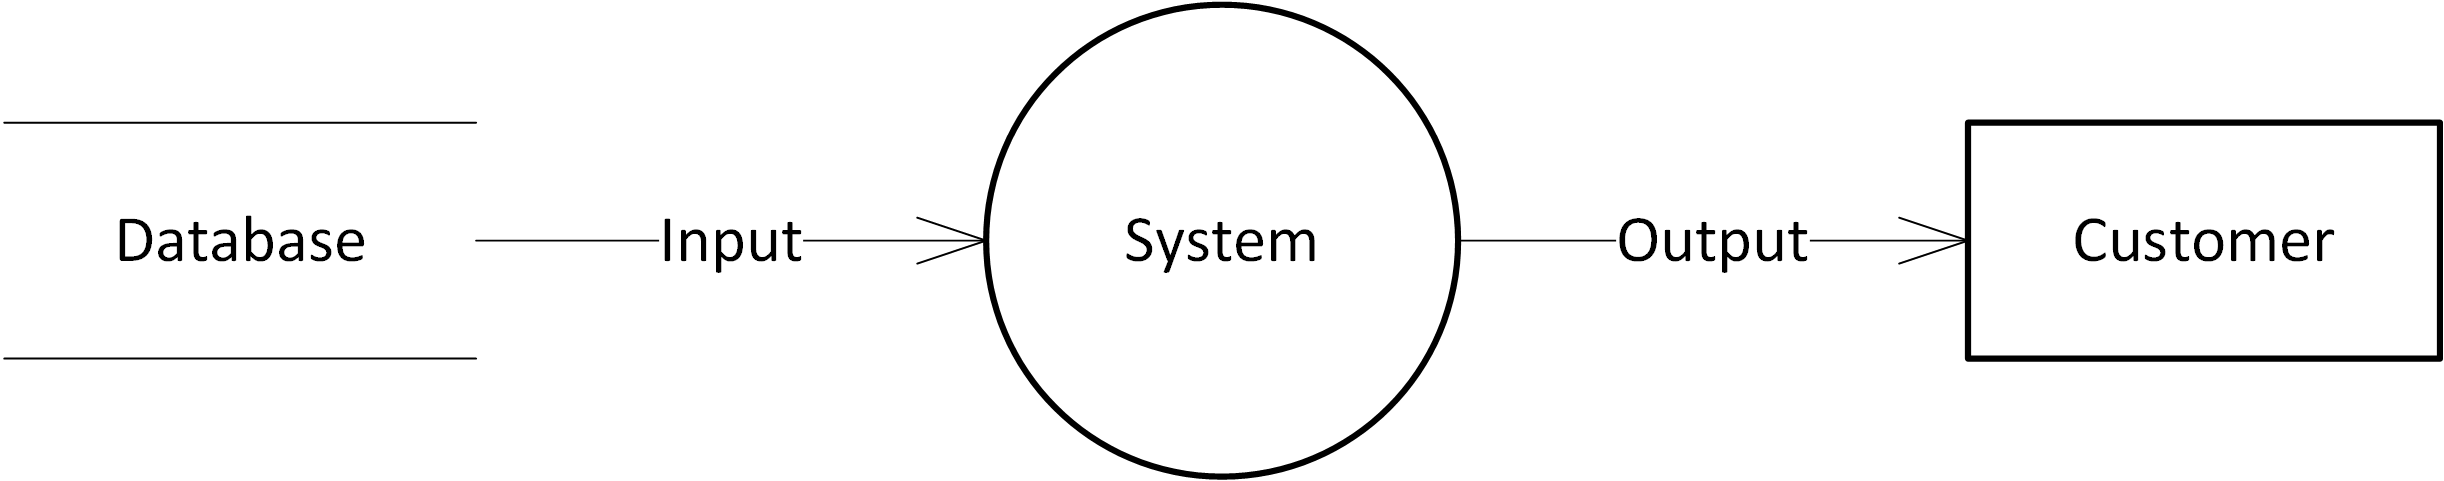
\includegraphics[width=0.8\textwidth]{images/datenflussdiagramm.png}
	\caption{Beispiel für ein Datenflussdiagramm}
	\label{img:datenflussdiagramm}
\end{figure}

\section{Informationsflussanalyse}
\label{sec:datenflussanalyse}
Die Modelle, die im Verlauf der Bachelorarbeit entstehen, sollen später als Eingabe für Datenflussanalysen dienen. Deshalb sind Arbeiten relevant, die sich mit Datenflussanalysen beschäftigen. Daraus können Anforderungen abgeleitet werden, die für die Modellierung benötigt werden. Im Folgenden sollen solche Arbeiten betrachtet werden. \par
Eine dieser Grundlagenarbeiten ist das Buch \textbf{Principles of Program Analysis} \cite{Basili1984}. In dieser Arbeit werden Datenflussanalysen auf Implementierungsebene beschrieben. Das heißt, dass um die Analyse ausführen zu können, eine Implementierung des Systems vorhanden sein muss. Die Datenflussanalyse wird mithilfe von Constant-Propagation, formuliert. Damit ist gemeint, dass konstante Ausdrücke zur Kompilierzeit ausgewertet werden. Ein Beispiel dafür ist in \autoref{img:constant_propagation} abgebildet. Dort werden die Kontrollkonstrukte statisch, zur Kompilierzeit, ausgewertet. 

\begin{figure}[h]
	\centering
  	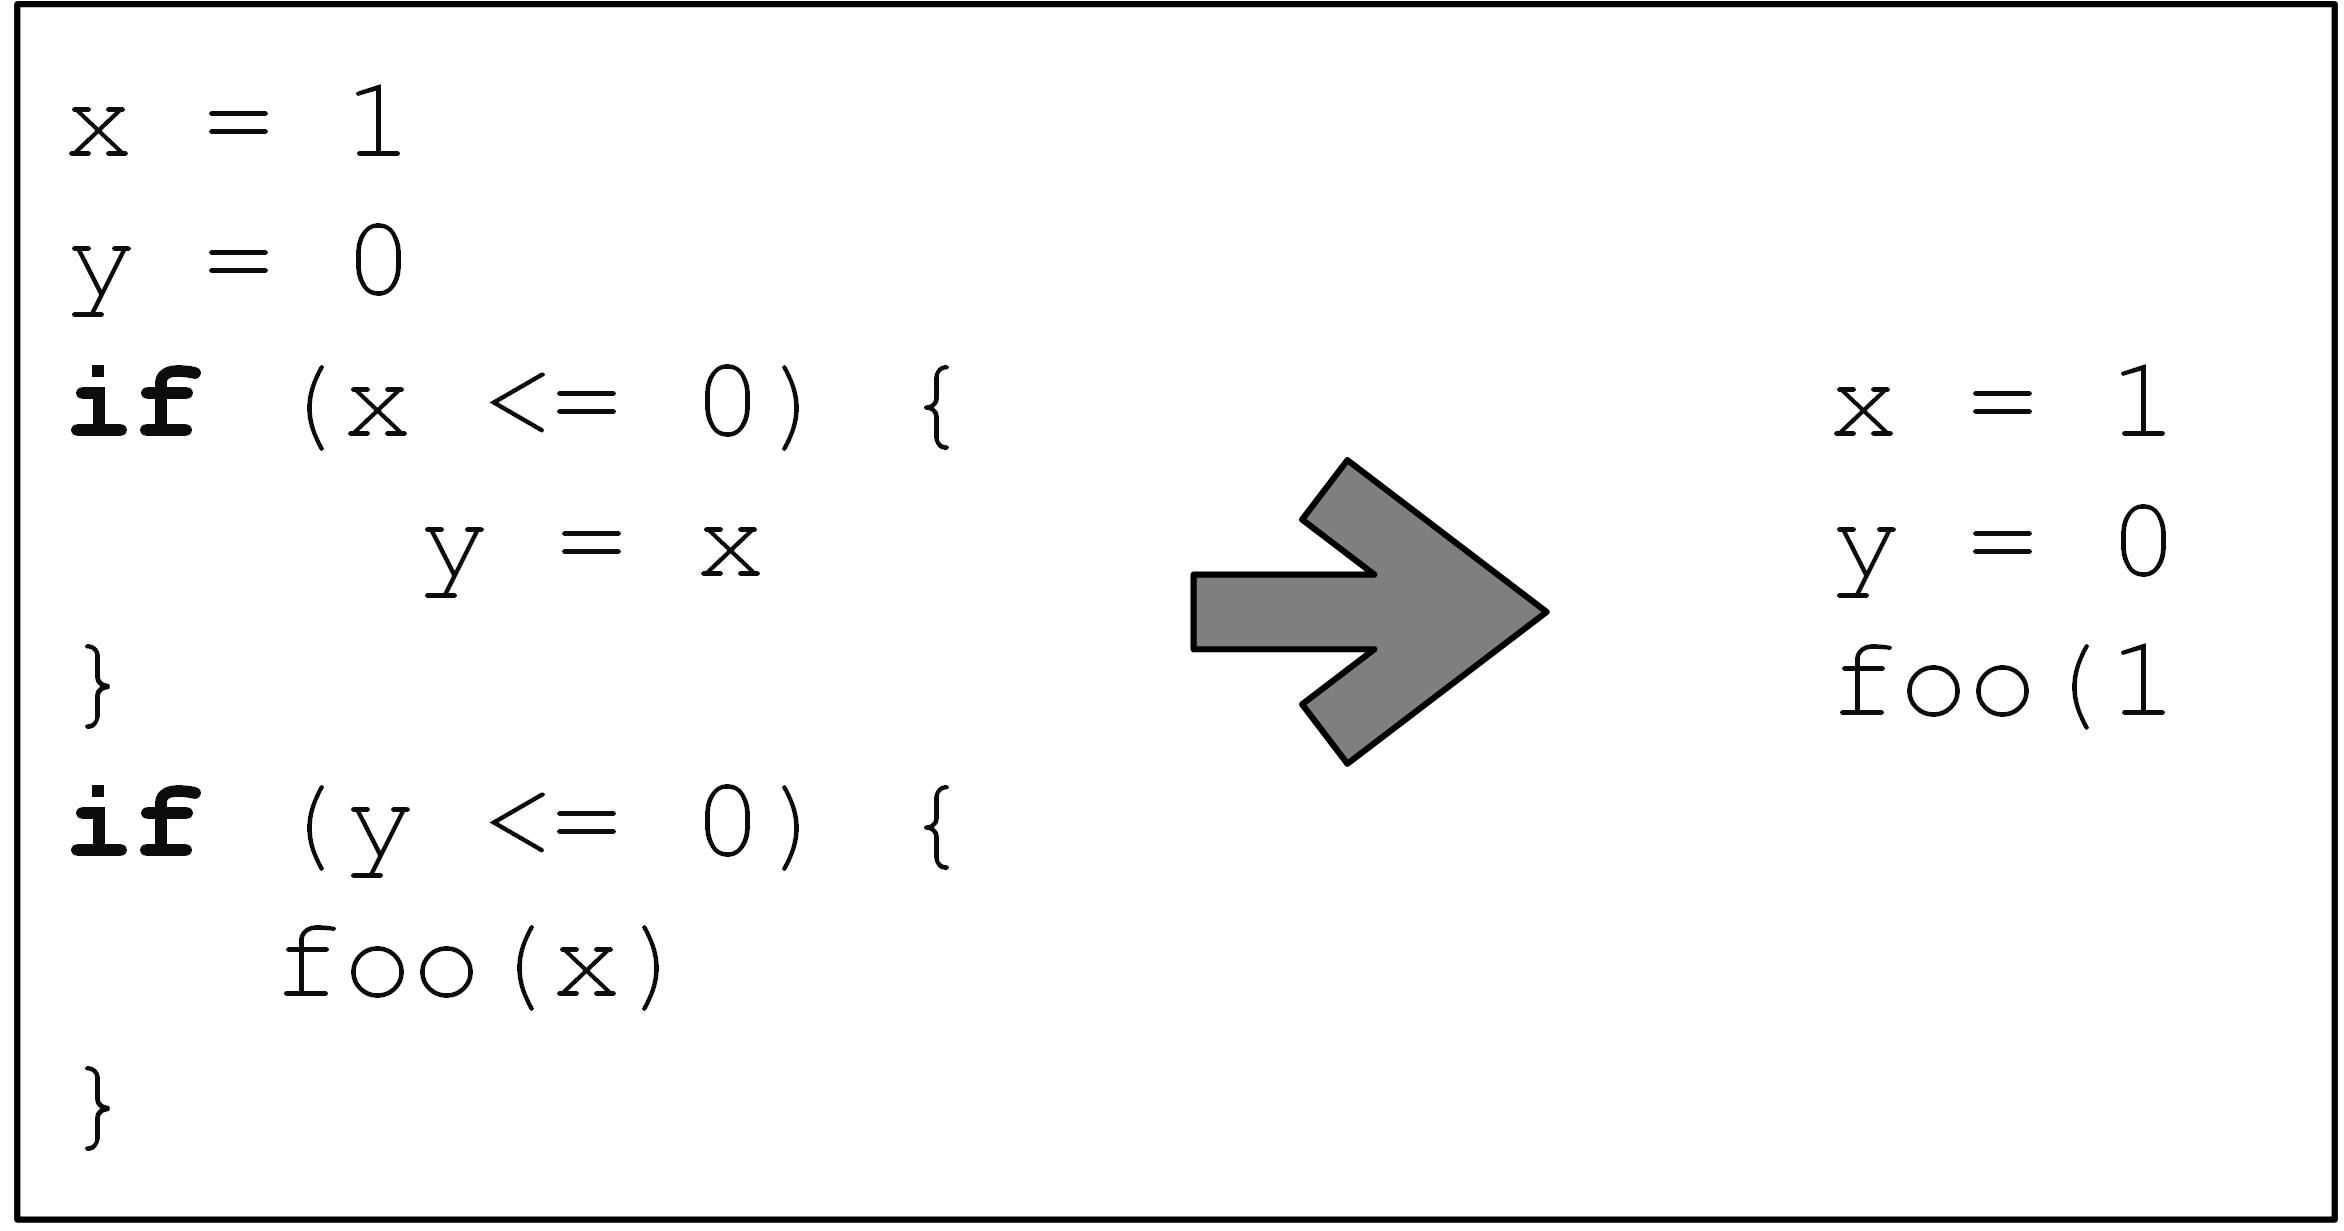
\includegraphics[width=0.7\textwidth]{images/cfg_code.png}
	\caption{Beispiel für Constant-Propagation}
	\label{img:constant_propagation}
\end{figure}

Der Ausgangspunkt für die Analyse ist dabei der \gls{cfg}. Ein \gls{cfg} besteht aus:
\begin{itemize}
\item Einer Menge von Knoten, die Instruktionen darstellen.
\item Einem Wurzelknoten, mit dem die Ausführung beginnt.
\item Einer Menge von gerichteter Kanten, die mögliche Programmabläufe darstellen.
\end{itemize}
In \autoref{img:cfg} ist der \gls{cfg} für das Beispiel aus \autoref{img:constant_propagation} abgebildet. Dabei werden in die Knoten eine oder mehrere Anweisungen des Codes eingetragen. Mit diesem \gls{cfg} kann im Anschluss eine Datenflussanalyse durchgeführt werden. \par
\begin{figure}[h]
	\centering
  	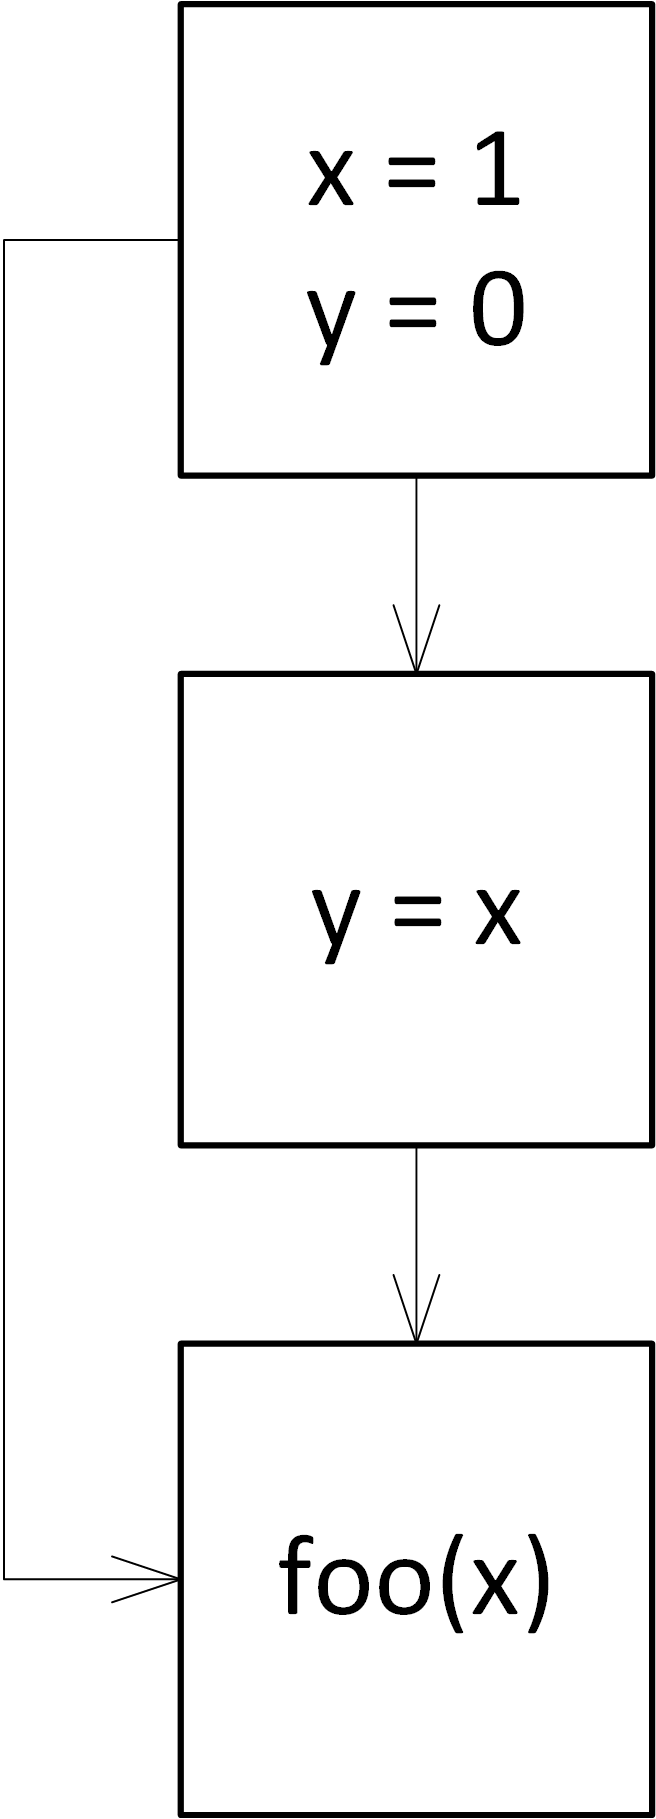
\includegraphics[width=0.16\textwidth]{images/cfg.png}
	\caption{Beispiel eines CFG, für das Beispiel aus \autoref{img:constant_propagation}}
	\label{img:cfg}
\end{figure}
Diese Analyse arbeitet jedoch nicht auf Datenflüssen, sondern leitet diese aus dem Kontrollfluss ab. Außerdem setzt die Analyse eine fertige Implementierung vorraus. In dieser Bachelorarbeit sollen Datenflüsse auf Architekturebene betrachtet werden. Dabei soll die Analyse direkt auf diesen Datenflüssen arbeiten und diese nicht aus dem Kontrollfluss ableiten. Deshalb soll im Weiteren nicht näher auf diese Arbeit eingegangen werden. \par 
In der Arbeit von Jürjens et al. \cite{Jurjens2005} wurde \textbf{UMLsec} vorgestellt. Dabei handelt es sich um eine Erweiterung für UML. \textbf{UMLsec} definiert 21 Stereotypen, die UML um Sicherheitseigenschaften erweitern. Ein Beispiel für einen Stereotypen, ist \texttt{Encrypted}. Mit diesem Stereotypen kann eine verschlüsselte Verbindung modelliert werden. Eine Sicherheitsanalyse kann im Anschluss mithilfe eines definierten Angreifers prüfen, ob das System sicher ist. Auch hier werden Datenflüsse nicht direkt verwendet, sondern aus dem Kontrollfluss abgeleitet. Da die Erweiterung für UML konzipiert ist und im Vordergrund der Arbeit die Sicherheit eines Systems und nicht der Datenfluss steht, wird sie im weiteren Verlauf der Bachelorarbeit nicht weiter betrachtet. \par
Eine Arbeit, die sich mit Datenflüsse auf Architekturebene befasst, ist die bereits in \autoref{sec:palladioerweiterungen} vorgestellte Arbeit \textbf{Model-Driven Specification and Analysis of Confidentiality in Component-Based Systems} \cite{Kramera}. Sie erweitert das \gls{pcm} um Datenflüsse und eine Vertraulichkeitsanalyse. Die Arbeit basiert auf dem Poster \textbf{Specification and Verification of Confidentiality in Component-Based Systems} \cite{Kramer}. Datenflüsse werden aber nicht innerhalb der Komponenten betrachtet. Außerdem werden Datenflüsse aus dem Kontrollfluss abgeleitet. Stattdessen werden Anforderungen für das Verhalten der Datenflüsse spezifiziert und anschließend überprüft. Die Prüfung der Komponente erfolgt zur Implementierungszeit auf Basis des Quelltexts. Die Arbeit beschreibt außerdem eine Vertraulichkeitsanalyse für Palladio. Diese Analyse prüft die Vertraulichkeit in komponentenbasierten Systemen. Für die Analyse müssen Eingabe und Ausgabe eines Systems spezifiziert werden, sowie Zugriffsspezifikation für Hardware und Kommunikationsverbindungen. Mithilfe dieser Informationen und einem Angreifer Modell, wird eine Architektur- und Code-Analyse durchgeführt. Nach Durchführung der Analyse werden Designfehler, Datenlecks und Verstöße gegen die Spezifikation angezeigt. Die Vertraulichkeitsanalyse hält sich ebenfalls an die Definition von Vertraulichkeit nach Eckert \cite{Eckert2013}. \par
In allen vorgestellten Arbeiten werden Eigenschaften für Daten festgemacht. Jedoch werden die Datenflüsse aus Kontrollflüssen abgeleitet. In dieser Bachelorarbeit sollen Daten und Datenflüsse als Objekte erster Klasse eingeführt werden. Für die Validierung soll jedoch die Vertraulichkeitsanalyse aus \cite{Kramer2012} verwendet werden, da diese bereits eine funktionierende Vertraulichkeitsanalyse für Palladio anbietet.

\section{Erweiterung des PCM}
Die Erweiterung des PCMs erfolgt durch die Erweiterung seines Meta-Modells. Dazu wurde von Strittmatter et al. \cite{Strittmatter} ein Ansatz entwickelt, bei dem die zu modellierenden Informationen in Gruppen eingeteilt werden. Das Meta-Modell wird in Schichten eingeteilt, die jeweils eine Gruppe abbilden. Schichten referenzieren sich gegenseitig. Dies führt zu einer modularen, flexiblen und erweiterbaren Struktur, die die Koexistenz von verschiedenen Qualitätsattributen und -analysen ermöglicht. Das Meta-Modell ist in die folgenden vier Schichten unterteilt:
\begin{itemize}
\item Die \textbf{Paradigm}-Schicht ist die Basisschicht. Sie legt den Grundstein für die Modellierungssprache, indem sie die Struktur, aber keine Semantik bereitstellt.
\item Die Semantik für die abstrakte Struktur der Sprache liefert die \textbf{Domain}-Schicht.
\item In der \textbf{Quality}-Schicht werden Qualitätseigenschaften für bestimmte Bereiche hinzugefügt.
\item Schließlich bietet die \textbf{Analysis}-Schicht Module für die Eingabe, Ausgabe und den internen Zustand. Außerdem gibt es Konfigurationsoptionen für Analysen.
\end{itemize}
Diese Arbeit wird für die Modellierung in \autoref{ch:modellierung} verwendet.
